\section{Artificial Neural Networks (ANN)}

\textcolor{blue}{Principals and basic feed forward networks}

\r{The most computationally expensive component is calculating the gradient of the loss function with respect to the parameters of the network}

% see page 233 of Understanding Machine Learning
\r{Artificial neural networks are {universal approximators}\index{universal approximators} -- \textcolor{red}{expand}}

\r{universal approximation theorem \textcolor{green}{(Hornik 1989, Cybenko, 1989)}. Regardless of the function that is attempted to being learned, a large MLP will be able to \textbf{represent} this function. However, it is not guaranteed that the large MLP, despite being a universal \textcolor{red}{approximator} capable of representing the function, is able to \textit{learn} the function}


\subsection{Multi-layer Perceptron}

\r{surprisingly/dangerously robust to bugs}

\r{Not a single multi-layer perceptron with multiple layers, rather it is a network composed of multiple layers of perceptrons. Multi-layer perceptrons, through use of sucessive transformations (multipel layers of adaptive weights) address some of the limitations presented with a single layer perceptron \TD{local ref}.  MLPs, even composed of just two layers, are capable of approximating any continuous functional mapping --- the restriction being that the network must be feed-forward (described in \TD{local ref}) ensuring the outouts are possible to calcualted from as explicit functions of the inputs.}

\r{universal approximator\cite{hornik1991approximation}}

\r{justification for deeper networks --- can be exponentially more compact.}

\subsection{Architecture}

\r{{input layer}\index{input layer}, {hidden layer}\index{hidden layer}, {output layer}\index{output layer}}

\r{the input layer is not counted in the number of layers in a network}

\begin{figure}[htp]
	\centering
	\includegraphics[width=0.5\textwidth]{example-image-a}\hfil
	\caption{\TD{TODO: diagram of neural network showing layers}}
	\label{fig:foundations_ann_overview}
\end{figure}


\subsection{Components}

\begin{figure}[htp]
	\centering
	\includegraphics[width=0.5\textwidth]{example-image-a}\hfil
	\caption{\TD{TODO: labeled diagram of nodes (weights and biases), connections, activation functions}}
	\label{fig:foundations_ann_overview}
\end{figure}


\subsubsection{Nodes / units}

\paragraph{Initialization}

\TD{TODO: initialization methods and for different layers}


\subsubsection{Activation Function}

\TD{TODO: I think this is where I'll talk about activation functions}

%% need for non-linearity
\r{If all the activation functions in the hidden layers of the network were to be linear then it is possible to create a equivalent network without the hidden units. This is due to the principle that the composition of successive linear transformations is itself a linear transformation \TD{show + detail more clearly}. \textcolor{red}{the activation functions of the hidden and output layers may be different.}}

\TD{TODO: step function to sigmoid function -- smoothed version of the step function -- can understand how an input changes the output.}

\r{When considering networks only consisting of threshold activations, we run into the {credit assignment}~\index{credit assignment problem} during training. That is we have no way of determining which of the hidden units is more/less responsible for the incorrect output.  A solution to this issue is to use differentiable activation functions, this then allows for the activation of the output to become differentiable functions of both the input variables and the parameters (weights and biases).}

%% TODO: placement
\r{A sigmoidal hidden unit can be used to approximate a hidden linear unit by scaling the input parameters (weights and biases) to be very small such that the values are small and lie on the linear part of the sigmoidal curve near the origin. Similarly a step function may be approximated by scaling the input parameters (weights and biases) to be very large such that the values are either in the activated or not activated state. Nearly any continuous functional mapping can be represetned by a network consisting of two layers of sigmoidal hidden units.  A network consisting of three or more sigmoidal hidden units can approximate any smooth mapping \TD{Lapedes and Farber 1988}}

\TD{local ref to a more in depth discussion of activation functions.}

%% this likely doesn't belong here
\begin{figure}[htp]
	\centering
	\includegraphics[width=0.3\textwidth]{example-image-a}\hfil
	\includegraphics[width=0.3\textwidth]{example-image-b}\hfil
	\includegraphics[width=0.3\textwidth]{example-image-c}\hfil
	\caption{\TD{TODO: three images of possible decision boundaries created by NN with threshold act.fn and 1,2, and 3 layers. one is a single linear hyperplane, 2 is a non convex and 3 is a disjoint}}
	\label{fig:foundations_ann_layers_decision_region}
\end{figure}

\r{networks having three or more layers of weights can create non-convex and disjoint decision regions. \TD{see Huang and Lippmann 1988 for examples of 2 layers.}. Networks with two layers are not capable of creating arbitrary decision boundries \TD{Gibson and Cownan 1990, Blum and Li, 1991} (also see \TD{fig ref}). However, if the activation function is converted to a sigmoidal activation, it is possible to arbitrarily closely approximate an given decision boundry.}

%%%%%%%%%%%%%%%%%%

\textcolor{blue}{Activation functions are XXXXXXXX}

\subsubsection{Why Non-linear}

\textcolor{blue}{Non-linear is necessary XXXXXXXXXX}


\subsubsection{Popular Activation Functions}

\r{Activation functions can be grouped into two main categories -- smooth and not smooth. Smooth activation functions (such as sigmoid) are differentiable at every point along the function where as the other activation functions are not differentiable at every location (relu).}

% history
%differentiable everywhere, monotonic, and smooth.


\r{linear (see above), }

\textcolor{blue}{ReLu, better because \textcolor{red}{help prevent saturation}, but still have problems \textcolor{red}{can "die" at 0.} }

\textcolor{blue}{ELU fuctions. they prevent the "dying" problem by being \textcolor{red}{non-zero} but their main drawback is that they are more computationally expensive due to the calculation of the exponent.}

\paragraph{Smooth Non-linear}

\subparagraph{Sigmoid}

\textcolor{blue}{The sigmoid\index{sigmoid} activation function.}

\textcolor{blue}{calibrated probability estimate}


% {{{act_smooth_sigmoid}}}
\begin{figure}
	\centering
	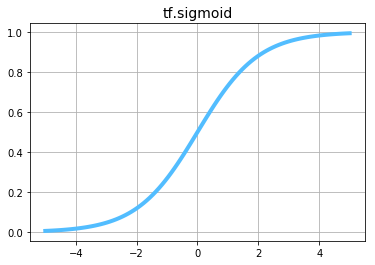
\includegraphics[width=0.65\textwidth]{./sync_imgs/act/smooth/sigmoid.png}
	\label{fig:act_smooth_sigmoid}
\end{figure}

% {{{act_smooth_tangent}}}
\begin{figure}
	\centering
	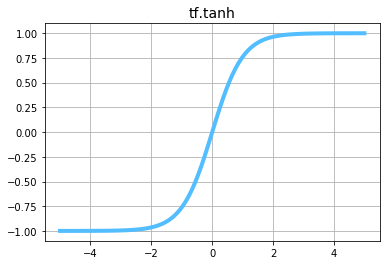
\includegraphics[width=0.65\textwidth]{./sync_imgs/act/smooth/tangent.png}
	\label{fig:act_smooth_tangent}
\end{figure}

\subparagraph{ELU}

\textcolor{blue}{\textcolor{red}{CITE}. Smooth, monotonic, and non-zero in the negative portion of the input. The main drawback is that they are more computationally expensive (due to calculating the exponential)}


\begin{equation}
{
	ELU = f(x) = \left\{
	\begin{array}{ll}
	\alpha(e^x - 1) x & \quad $for$ \ x < 0 \\
	x & \quad $for$ \ x \ge 0
	\end{array}
	\right.
}
\label{eq:act_elu_def}
\end{equation}


% {{{act_smooth_elu}}}
\begin{figure}
	\centering
	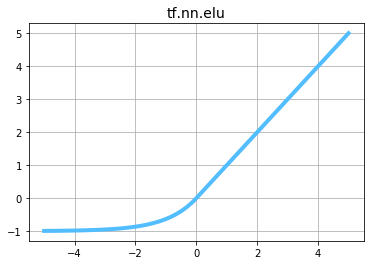
\includegraphics[width=0.65\textwidth]{./sync_imgs/act/smooth/elu.png}
	\label{fig:act_smooth_elu}
\end{figure}

% {{{act_smooth_selu}}}
\begin{figure}
	\centering
	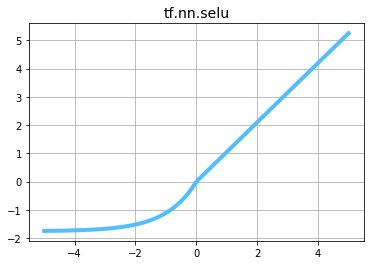
\includegraphics[width=0.65\textwidth]{./sync_imgs/act/smooth/selu.png}
	\label{fig:act_smooth_selu}
\end{figure}


\subparagraph{Softplus}

\textcolor{blue}{continuous and differentiable at zero. However, due to the natural log and exponential function, there is added computation compared to th ReLU.}

% typcially discouraged in practice since ReLU achieves similar results and is less computationally expensive

\begin{equation}
{
	Softplus = f(x) = \ln{(1+e^x)}
}
\label{eq:act_softplus_def}
\end{equation}


% {{{act_smooth_softplus}}}
\begin{figure}
	\centering
	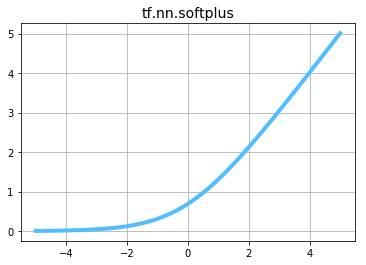
\includegraphics[width=0.65\textwidth]{./sync_imgs/act/smooth/softplus.png}
	\label{fig:act_smooth_softplus}
\end{figure}

% {{{act_smooth_softsign}}}
\begin{figure}
	\centering
	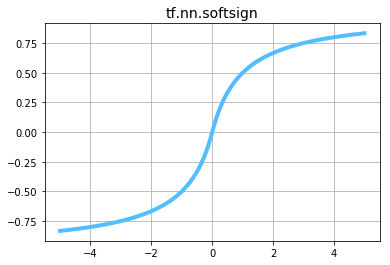
\includegraphics[width=0.65\textwidth]{./sync_imgs/act/smooth/softsign.png}
	\label{fig:act_smooth_softsign}
\end{figure}


\paragraph{Not Smooth Non-linear}

\subparagraph{ReLU}

\begin{equation}
{
	ReLU = f(x) = \left\{
	\begin{array}{ll}
	0 & \quad $for$ \ x < 0 \\
	x & \quad $for$ \ x \ge 0
	\end{array}
	\right.
}
\label{eq:act_relu_def}
\end{equation}

% {{{act_notsmooth_relu}}}
\begin{figure}
	\centering
	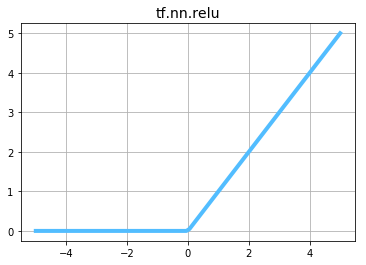
\includegraphics[width=0.65\textwidth]{./sync_imgs/act/notsmooth/relu.png}
	\label{fig:act_notsmooth_relu}
\end{figure}

\subparagraph{Leaky ReLU}

\textcolor{blue}{The Leaky ReLU (Eq~\ref{eq:act_leaky_relu_def}) was designed in attempt to address the dying ReLU issue \textcolor{red}{CITE}. Rather than simply outputting a zero in the negative range, the Leaky ReLU will will have a small non-zero slope (user specified) -- allowing weight updating and training to continue.}

\textcolor{green}{TODO: randomized Leaky ReLU \textcolor{red}{cite} --- $\alpha$ (from PReLU) is sampled from a uniform distribution randomly. The net-effect could be considered similar to drop out since, technically, there is a different network for each value of $\alpha$, resulting in an ensemble of sorts. At test time, the values for $\alpha$ are averaged.}

\begin{equ}[!ht]
	\begin{equation}
	{
		Leaky ReLU = f(x) = \left\{
		\begin{array}{ll}
		N x & \quad $for$ \ x < 0 \\
		x & \quad $for$ \ x \ge 0
		\end{array}
		\right.
	}
	\label{eq:act_leaky_relu_def}
	\end{equation}
	\caption{where $N$ is a constant. $N$ is typically set to 0.01}
\end{equ}

% {{{act_notsmooth_leakyrelu}}}
\begin{figure}
	\centering
	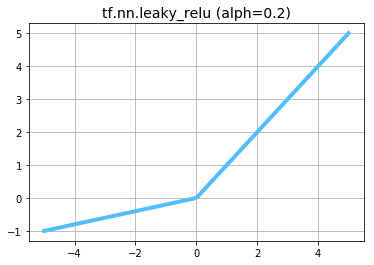
\includegraphics[width=0.65\textwidth]{./sync_imgs/act/notsmooth/leakyrelu.png}
	\label{fig:act_notsmooth_leakyrelu}
\end{figure}

\subparagraph{ReLU6}

\textcolor{blue}{In general, this function is referred to as a {ReLUN}\index{ReLUN} function, where $N$ is some constant. However, in practice, $6$, was determined to be the optimal value.\textcolor{red}{CITE}. \textcolor{red}{This capped value, may help learn the sparse values sooner.} By having the upper limit bounded, the prepare the network for a fixed point precision for inference --- if the upper limit is unbounded, then you may loose too many bits to \textcolor{red}{Q} portion of the fixed point number.}


\textcolor{blue}{Similar to the ReLU fuction, only the output is capped to six in the positive domain.}

\begin{equation}
{
	ReLU6 = f(x) = min{(max{(0,x)},6)}
}
\label{eq:act_ReLU6_def}
\end{equation}

% {{{act_notsmooth_relu6}}}
\begin{figure}
	\centering
	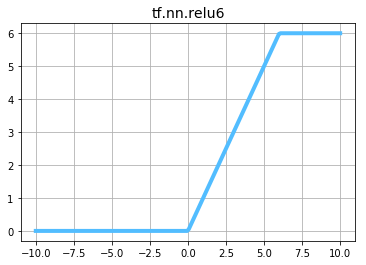
\includegraphics[width=0.65\textwidth]{./sync_imgs/act/notsmooth/relu6.png}
	\label{fig:act_notsmooth_relu6}
\end{figure}

\subparagraph{PReLU}

\begin{equ}[!ht]
	\begin{equation}
	{
		PReLU = f(x) = \left\{
		\begin{array}{ll}
		\alpha x & \quad $for$ \ x < 0 \\
		x & \quad $for$ \ x \ge 0
		\end{array}
		\right.
	}
	\label{eq:act_prelu_def}
	\end{equation}
	\caption{where $\alpha$ is a parameterized --- a learned parameter from training.}
\end{equ}

\r{Parametric Rectified Linear Unit (PReLU) \cite{he2015delving}}

\textcolor{blue}{$\alpha$, rather than being hard coded, is determined during training by the data. The logic being that the value would be more optimal than we could set \textcolor{red}{CITE}}

% {{{act_notsmooth_prelu}}}
\begin{figure}
	\centering
	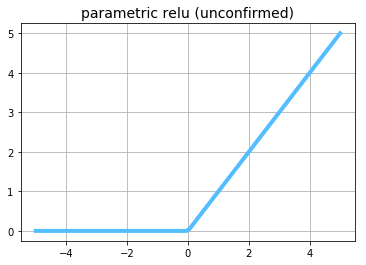
\includegraphics[width=0.65\textwidth]{./sync_imgs/act/notsmooth/prelu.png}
	\label{fig:act_notsmooth_prelu}
\end{figure}


\TD{Self-Normalizing Neural Networks \cite{DBLP:journals/corr/KlambauerUMH17}}




%%%%%%%%%%%%%%%%


\subsection{Characterization}

\subsubsection{Types: Feed-forward vs Feedback}

\textcolor{blue}{Feed-forward --- Directed acyclic graph of artificial neurons. Feedback contain feedback connections that are fed back into itself. When feedforward are include these feedback connections, they become considered recurrent neural networks.}

\paragraph{Feed-forward}

\r{``general framework for representing non-linear functional mappings between a set of input variables and a set of output variables''}

\subparagraph{Layered networks}

\begin{figure}[htp]
	\centering
	\includegraphics[width=0.5\textwidth]{example-image-a}\hfil
	\caption{\TD{TODO: layered network diagram}}
	\label{fig:foundations_ann_layered_network}
\end{figure}

\r{Whereas a single layer network is composed of linear combination of input variables, that are then, transformed by a non-linear activation function, more general functions are creating layered networks that are composed of successive layers of processing units (adaptive weights) with connections running from every unit in one layer to every unit in the next.}

\subparagraph{General topologies}

\begin{figure}[htp]
	\centering
	\includegraphics[width=0.5\textwidth]{example-image-b}\hfil
	\caption{\TD{TODO: general topology}}
	\label{fig:foundations_ann_general_topology}
\end{figure}

\r{general topologies}

\paragraph{Feedback}

\subsubsection{Terminology}

\r{Considered \textit{networks} since they are typically composed of many different functions --- creating a ``network''.}

\r{Considered \textit{neural} since they are \textbf{loosely} inspired by neuroscience.}

\r{layer --- a layer may be considered a group of units that act in parallel. The layer will extract representations from the input, that are (in theory) more useful to the specific task.  Chaining together these layers results in a form of progressive \IDI{data distillation}.}

\r{Visible and Hidden Layers. Visible layers are called visible since they contain variables that are ``visible'', where as the hidden layers extract increasingly abstract features -- hidden since their values are not given in the raw data, but rather an output from a previous layer.}



\subsection{Learning: Backpropagation}

% see p196[184] of Mastering ML w/SKL
\TD{TODO: whoooo, this is going to be a big one. understand how each component contributes to the error and adjust accordingly.}

\r{popularized by \TD{Rumelhard, Hinton and Williams (1986)}, but similar ideas were discussed earlier by \TD{Werbos 1974}, and \TD{Parker 1985}}

\r{error backpropagation is used for evaluating the dervivatives of an error function with respect to the parameters (weights and biases) of the network}

\r{Iterative algorithm consisting of two main components --- the forward, then reverse, pass.}

% see p.141(156) - 146(161) of NNbishop
\TD{MORE}

\TD{Example}

\paragraph{Forward pass}

\r{In the forward pass inputs are propagated through the network and derivatives of the error functuion, with respect to the parameters (weights and biases) are evaluated. Propagation o ferrors through the network, calculating the derivatives, can be applied to may different error functions.}

\r{it becomes important to use a computationally efficient method for evaluating these derivatives \TD{local ref}}

\r{During this stage is when the errors are propagated through the network.}

\paragraph{Backward pass}

\r{In the Backward pass, the previously calcuated derivatives are used to compute the adjustments to the parameters --- propagated in reverse through the network (from cost function to input layer) and each node is updated -- \TD{TODO: expand}.}

\r{backpropagation\cite{alber2018backprop}}

\r{Many optimization schemes \TD{local ref} may be used to adjust the parameters by using the calculated derivatives from the forward pass.}

\r{The calculated derivatives are used by the majority of training algorithms}

%% p116 of neural networks, p131 on tablet
\TD{Hessian matrix is a matrix containing the second derivative of a function. The second derivative provides information about the curvature of the function.}

% see p197-201[180] of Mastering ML w/SKL
\TD{TODO: figure showing sample calculation}


% See p207 of DL



\r{\IDI{symbolic differentiation} --- compute a gradient function for the chain (chain rule) mapping parameter values to gradient values}

\subsubsection{Back-propagation efficiency}

%% see para in p146(161) of bishop NN

\subsubsection{Chain Rule}

\r{See \textcolor{red}{local ref to math prereq section}}

\TD{TODO: chain rule}

\r{Backpropagation is typically used with an optimization algorithm (see \textcolor{red}{local ref?})}

\subsection{Autodiff}

\TD{Autodifferentiation (\IDI{autodiff})}

\begin{itemize}[noitemsep,topsep=0pt]
	\item Manual differentiation
	\item Finite difference approximation
	\item Autodiff
	\begin{itemize}[noitemsep,topsep=0pt]
		\item Forward-mode autodiff
		\item Reverse-mode autodiff
	\end{itemize}
\end{itemize}

\TD{automatic differentiation may be used to estimate derivatives numerically as the derivative is not always known.}

\r{Tensorflow uses \IDI{reverse-mode differentiation}.  Calculate the contribution that each parameter had on the loss value}

\subsubsection{Manual differentiation}

\r{calculus ``by hand''}

\subsubsection{Finite difference approximation}

\r{using infinitely close points on a function to calculate the slope of line passing through these points.}

%TODO: very nice code example in hands on ML that is worth including here

\TD{specific equation, Newton's difference quotient}

\subsubsection{Forward-mode autodiff}

% TODO: same flaw as above, more accurate, but requires just as many passes -- which is ``unfeasible'' for large scale NN

\TD{dual numbers}

\subsubsection{Reverse-mode autodiff}

% TODO: only two passes needed

\subsection{Multi-layer perceptrons}

% TODO: this doesn't really belong here.. will need ot work on placement

\subsection{Operations}

\subsection{Convolution}
% TODO: I'm not sure how I'm going to structure these yet or where I'll be placing them

% TODO: https://arxiv.org/abs/1904.11486
% https://www.youtube.com/watch?v=HjewNBZz00w


\r{Convolutions are built upon a lie -- that is we refer to the opperation as a convolution, yet it is in fact a cross-correlation operation since we don't rotate the kernel 180$\deg$. However, it is convention to refer to the operation as a convolution. For more, please see section \ref{conv_vs_cross}}

\r{translational invariance --- a property that relates to how a systems decisions are insensitive to the location of a features within an input. That is, if we're looking for an object or feature, our system shouldn't change if the object is in different locations within the input}

\TD{Neocognitron -- CNN paper prior to ``CNN''\cite{fukushima1982neocognitron}}

% Survey on CNNs
% TODO: a lot here -- good read
\TD{A Survey of the Recent Architectures of Deep Convolutional Neural Networks \cite{DBLP:journals/corr/abs-1901-06032}}


\TD{Squeeze-and-Excitation Networks \cite{DBLP:journals/corr/abs-1709-01507}}


% Graham Taylor
\r{weighted averaging operation in time or space}


\r{translation equivariant --- }

\r{DNN on an image may not take advantage of the ``stationarity'' (statistics) of an image. Patterns don't depend on the spatial location.}

\r{spatial hierarchies --- \TD{TODO: figure raw data, abstract edges+, then more distinct images, then closer output to the output, then the final label}}

\textcolor{red}{local ref to TensorFlow implementation}

\r{typcially a feature extraction phase (consisting of convolutional and pooling layers) followed by a classifier block (dense layers).}

%%%% popular layer types
\textcolor{green}{TODO: feature maps, (height, width, and depth (also called channels axis)). Stride, filter size, depth. talk about parameters}

\r{The output feature map (every dimension in the depth axis is a feature/filter) --- after a convolution operation the depth of a layer is no longer representative of a color channel (like RGB), it is now representative of a feature extracted by the convolutional operation, these are called filters.}

\TD{Strided Convolution\cite{springenberg2014striving}}

\TD{Dilated Convolution --- `atrous' convolution. (famously used by wavenet), which is convenient in time series analysis.}

\r{weight tieing}


\textcolor{green}{TODO: figure}

\begin{figure}[htp]
	\centering
	\includegraphics[width=0.5\textwidth]{example-image-a}\hfil
	\caption{Figure example of convolution operation on 2d image \textcolor{green}{TODO}}
	\label{fig:conv_2d_example_calc}
\end{figure}

\begin{figure}[htp]
	\centering
	\includegraphics[width=0.5\textwidth]{example-image-b}\hfil
	\caption{Figure example of convolution operation on 3d image \textcolor{green}{TODO}}
	\label{fig:conv_2d_depth_example_calc}
\end{figure}

\textcolor{green}{TODO: examples of how different filter values and strides can effect the output dimensions.}




\subsection{Pooling}
% TODO: I'm not sure how I'm going to structure these yet or where I'll be placing them -- pooling really does not belong under feed forward

\TD{TODO: examples of max vs average pooling}

%%%%%% research
\textcolor{blue}{Pooling may not fully determine learned deformation stability -- possibly filter smoothness\cite{ruderman2018learned}}

\r{downsampling}

\r{Why? importance of reducing the number of params.}

\TD{L2-pooling}

\TD{L2-pooling over the features or channels.}

\TD{additional --- learned/parameterized pooling}

\begin{figure}[htp]
	\centering
	\includegraphics[width=0.5\textwidth]{example-image-a}\hfil
	\caption{Figure example of max pooling operation on 2d image \textcolor{green}{TODO: I want this figure to be basic 2d}}
	\label{fig:pooling_max_2d_ex_a}
\end{figure}

\begin{figure}[htp]
	\centering
	\includegraphics[width=0.5\textwidth]{example-image-b}\hfil
	\caption{Figure example of average pooling operation on 3d image \textcolor{green}{TODO: I want this figure to be 3d}}
	\label{fig:pooling_avg_3d_ex_a}
\end{figure}


\r{may be better to use convolutional layers in place of the pooling layers\cite{springenberg2014striving}}